\chapter{Merging the graph and the dictionary learning part}
\label{sec:GD}
\cri{nelle osservazioni aggiungi:
- Il criterio di scelta dell'inizailizzazione ---> Cerca di capire bene come viene inizializzato il dizionario per essere sicura che quello che stai dicendo nella sezione non è una cazzata
- Il fatto che l'inizializzazione non è così vincolante
- perchè ci sono disparità nel numero di iterazioni
- come varia il comportamento dell'algoritmo in base alla variazione dei parametri che abbiamo: del tipo, più samples vuol dire maggiore precisione ecc..}
The next step of our work focuses on the attempt to learn at the same time the Dictionary and the graph structure, while in a further moment we will focus on adding the previous smoothness constraint. As it is formulated theoretically, the double optimization problem could reveal itself to be heavily ill posed, since now the number of parameters involved in the optimization would go up to three instead of the already challenging two. To remedy the problem we decided to create an algorithm which alternates the dictionary learning and the graph learning step, while the sparsity prior is checked at every step by the continuous optimization of the sparsity matrix $X$.\\
\section{The initialization section}
In this situation, one first aspect we have to be careful about is how we initialize the elements for the optimization, namely $W$ and $D$, since both them are clearly necessary from the beginning. The choice is between initialising the kernels coefficients and initializing the graph structure: since each entity is strictly correlated with the other, one of the two can be reduced. Our hypothesis is that forcing some kind of structure in the kernels, even though random, could heavily influence the overall behavior of the optimization structure, since a small error in their estimation could easily propagate through the structures that develop onto them; on the other hand, initializing the graph structure in a random way would not bias our learning problem with the same importance. Moreover, the nature of the two learning parts is slightly different: in the dictionary learning part the algorithm attempts to find the only solution that could exist, while in the graph learning part the algorithm aims at finding a good solution for the problem, without necessarily meaning that the graph learned is the same as the ground truth one, since it just has to be one possible solution to the problem. Under this light, it is clear that the graph initialization has smaller consequences than the initialization of the kernels. In order to verify our reasoning we run some tests to see if the intuition was correct and the results aligned with it. \cri{mostrali nei risultati poi}.


Therefore, in this first part we initialize the weight matrix $W$, obtain the related normalized Laplacian $\mathcal{L}$ and compute the orthogonal basis connected to it on order to use the eigenvectors we find to have a first estimate on the dictionary.

\section{The alternation between optimization steps}
With this starting elements we are then able to pass to the alternating optimization steps: every iteration of the global cycle involves the sparsity matrix estimation $X$ through the \gls{omp} method (the so-called \textit{sparse coding step}), while what occur in turn every time are the \textit{dictionary learning} and the \textit{graph learning} steps. Finally, after the learning steps there is a re-estimation of the dictionary based on the new values of $\alpha$ and $\mathcal{L}$ which will then be used in the next iteration from the spars coding step. \cri{vedi se puoi spiegarlo un po' meglio}.

The general algorithm thus articulates in the following way:

\begin{algorithm}[H]
  \caption{Parametric dictionary and graph learning}
  \begin{algorithmic}[1]
    \Procedure{initialization}{}
      \State $Y \gets \text{Signal samples set}$
      \State $T_0\gets \text{Target sparsity}$
      \State $K \gets \text{Polynomial degree}$
      \State $S \gets \text{Number of subdictionaries}$
      \State $iterNum \gets \text{Number of iterations}$
      \State $W \gets \text{Random thresholded adjacency matrix}$
    \EndProcedure
    \For{$i=1,2,\dots, iterNum$}
      \Procedure{Sparsity step}{}
        \State $X \gets \text{Sparsity estimation with \gls{omp}}$
      \EndProcedure
      \Procedure{Learning step}{}
        \If{$mod(i,5) = 0$} \label{5}
          \State $\alpha \gets \text{kernels estimation through sdpt3}$
        \Else
          \State $W \gets \text{graph estimation through gradient descent}$
          \State $\mathcal{L} \gets D^{-\frac{1}{2}}LD^{-\frac{1}{2}}$
        \EndIf
      \EndProcedure
      \Procedure{Dictionary update step}{}
        \State $\mathcal{D} \gets \sum_{k=0}^K \alpha_k \mathcal{L}^k$
      \EndProcedure
    \EndFor
    \end{algorithmic}
\end{algorithm}

We specify that, as shown in the pseudo code at line \ref{5}, in our algorithm there is no equal distribution of the iterations dedicated to graph and dictionary learning, but there is a rate $5:1$ in favour of the graph learning. This choice was born from two main facts:
\begin{itemize}
\item While the dictionary learning procedure is converging to its minimums discretely fast, the graph learning part requires more steps for it, concluding that giving more space of action to it was a way to balance the optimization steps;
\item The sparsity step revealed to be more sensible to alterations of its inputs (the dictionary in our case) when those were due to the kernel coefficients (and so the dictionary learning step) in such a way that limiting these learning steps in their number was advisable;
\end{itemize}

\section{Results}
For the tests we run regarding this part, we deployed the same datasets used in \autoref{sec:dataGen}: a graph signal with edge weights taken from a gaussian distribution, a Heat kernel and the kernel isolated from Thanou et al. dataset.

Moreover, the number of iterations we chose is $iterNum = 250$, the sparsity factor still equal to $T_0 = 4$ and the coherence factor $\mu = 10^{-4}$.

Together with the representation error we added another metric to evaluate the quality of our approach, a function estimating the Precision and the Recall rate for the graph. To be precise, the Precision metric expresses the percentage of estimated edges in the graph that are correct, while the Recall metric shows the rate of the original edges are correctly estimated.\\
The experiments showed promising results, not particularly degraded by the alternating process.

In \autoref{fig:alphaHeatGD} and \autoref{fig:alphaDorinaGD} the original and the learned kernels are compared: as it can be seen from the figures, the learning process is not particularly affected  by the fact that at the beginning of our optimization procedure we have to suppose as unknowns both the graph structure and the dictionary coefficients. The only noticeable difference is in the absolute value of the kernels, as it is slightly reduced, and the spectral range of the eigenvalues: these ones are constantly updated at every graph learning step and the results indicate the tendency to "contract" the spectral range, bringing it further from the 0 value. The constraints over the dictionary, anyway, prevent the learned solution to be sensibly altered and assure the spectral distribution of the frequencies already assumed in the dictionary learning approach.

\begin{figure}
  \centering
  \begin{minipage}[c]{.8\textwidth}
    \centering
    \includegraphics[width = \textwidth]{comp_kernels_Heat30.png}
  \end{minipage}
  \begin{minipage}[c]{.8\textwidth}
    \centering
    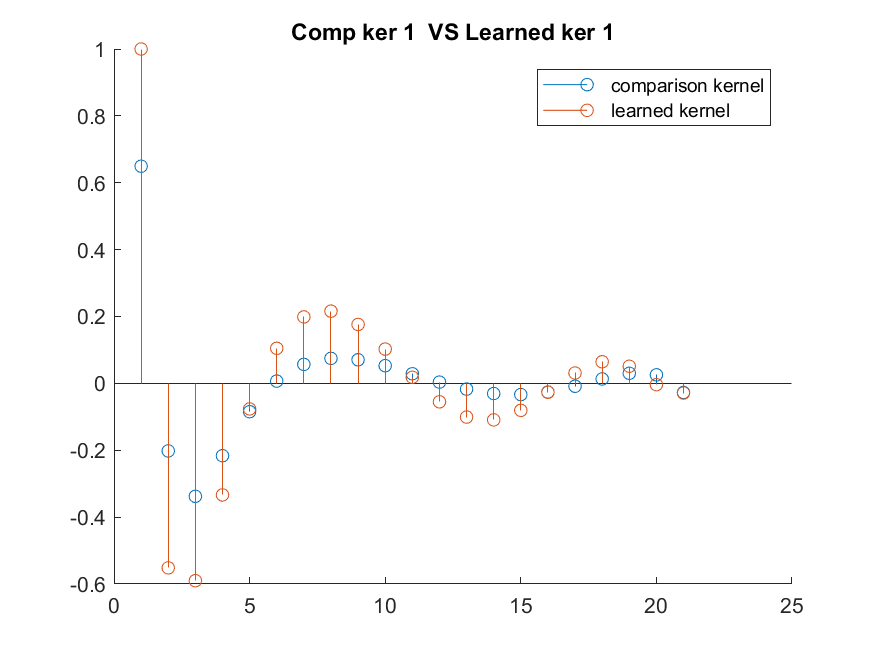
\includegraphics[width = \textwidth]{alphaDorina_Smoothness_dictionary.png}
  \end{minipage}
  \caption{Comparison between kernels coefficients without and with smoothness prior. Thanou et al.   dataset}
  \label{fig:alphaHeatGD}
\end{figure}

\begin{figure}
  \centering
  \begin{minipage}[c]{.8\textwidth}
    \centering
    \includegraphics[width = \textwidth]{comp_kernels_DorinaLF.png}
  \end{minipage}
  \begin{minipage}[c]{.8\textwidth}
    \centering
    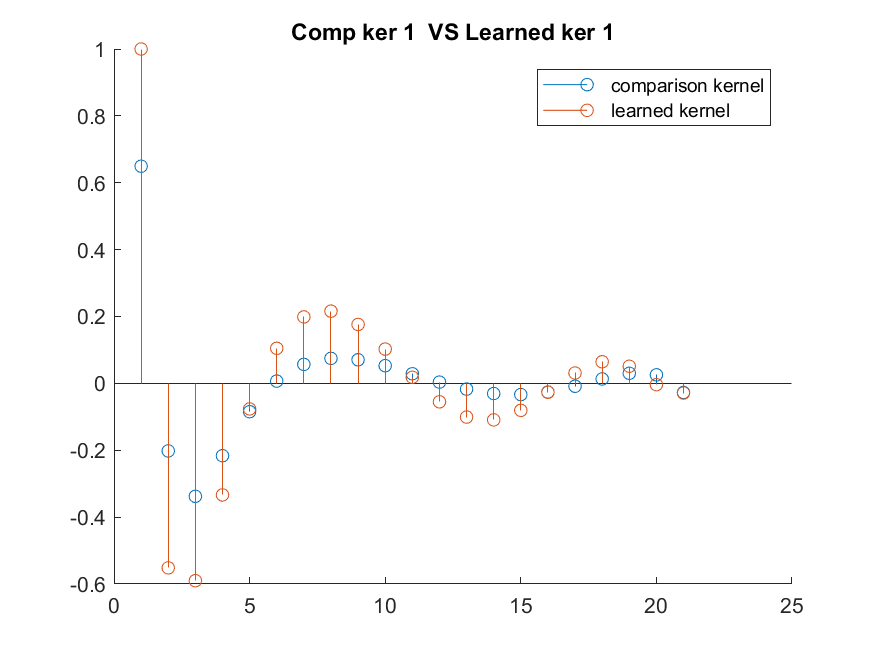
\includegraphics[width = \textwidth]{alphaDorina_Smoothness_dictionary.png}
  \end{minipage}
  \caption{Comparison between kernels coefficients without and with smoothness prior. Thanou et al.   dataset}
  \label{fig:alphaDorinaGD}
\end{figure}

\cri{mancano i kernels imparati corretamente dal'algo GD senza constraint}

In the \autoref{tab:PrecRec_noSmth} what is presented is the comparison between the Precision and Recall values obtained from the graph learning only approach and the approach combining graph and dictionary learning. The values listed confirm the fact that alternating between the two learning phases does not affect the single learning process significantly and remains feasible, even though we are doubling the aspects to take into account when optimizing

\begin{table}[htbp]
  \centering
  \begin{tabular}{lcccc}
  &\multicolumn{2}{c}{\textbf{Heat kernel}}&\multicolumn{2}{c}{\textbf{Thanou et al. kernel}}\\
  \toprule
  &Graph L. & Graph and D. L. & Graph L. & Graph and D. L.\\ %\cline{2-5}
    \midrule
    \textbf{Precision rate} & 0 & 0 & 0 & 0\\
    \textbf{Recall Rate} & 0 & 0 & 0 & 0\\
    \bottomrule
  \end{tabular}
  \caption{Reproduction error comparison for the low frequency kernel from Thanou et al. dataset}
  \label{tab:PrecRec_noSmth}
\end{table}

Finally, regarding the representation error the table \ref{tab:errorGD} shows how the learned dictionary is not significantly degraded in quality with respect to the dictionary-only learning algorithm, but still remains acceptable:

\begin{table}[htbp]
  \centering
  \begin{tabular}{lcccc}
  &\multicolumn{2}{c}{\textbf{Heat kernel}}&\multicolumn{2}{c}{\textbf{Thanou et al. kernel}}\\
  \toprule
  &Dictionary L. & Graph and D. L. & Dictionary L. & Graph and D. L.\\ %\cline{2-5}
    \midrule
    \textbf{Avg. repr. Error} & 0 & 0 & 0 & 0\\
    \bottomrule
  \end{tabular}
  \caption{Reproduction error comparison for the low frequency kernel from Thanou et al. dataset}
  \label{tab:errorGD}
\end{table}
